\documentclass{article}

\usepackage[utf8]{inputenc}
\usepackage[T1]{fontenc}
\usepackage{microtype}

\usepackage{newspaper}

\date{\today}
\currentvolume{1}
\currentissue{1}

%% [LianTze] The newspaper package also provides 
%% these commands to set various metadata:

%% The banner headline on the first page
%%   (The colon after s: is to get a more
%%   modern majuscule s in this font instead of 
%%   the medieval tall s. For anyone interested 
%%   in the history: 
%%  http://medievalwriting.50megs.com/scripts/letters/historys.htm)
\SetPaperName{Math Chronicles:}

%% The name used in the running header after
%% the first page
\SetHeaderName{Committee Times}

%% and also...
\SetPaperLocation{Bassano del Grappa}
\SetPaperSlogan{``All the News I Feel Like Printing.''}
\SetPaperPrice{ZenMaths}


% [LianTze] times (the package not the font) is rather outdated now; use newtx (see later)
% \usepackage{times}
\usepackage{graphicx}
\usepackage{multicol}

\usepackage{picinpar}
%uasage of picinpar:
%\begin{window}[1,l,\includegraphics{},caption]xxxxx\end{window}


%% [LianTze] Contains some modifications
\usepackage{newspaper-mod}
%%... so now you can redefine the headline and byline style if you want to.
%% These can be issued just before any
%% byline or headline in the paper, to
%% individually style each article
%%
% \renewcommand{\headlinestyle}{\itshape\Large\lsstyle}
% \renewcommand{\bylinestyle}{\bfseries\Large\raggedright}


%%%%%%%%%  Front matter   %%%%%%%%%%

\usepackage{lipsum}

\begin{document}
\maketitle

\begin{multicols}{3}

\byline{Geek Designs New \LaTeX{} Package}{Matthew Allen}

The package is basically a redefinition of the \verb+\maketitle+ command.  The model was the New York Times---hopefully I haven't violated any copyright laws.  I also had to redefine the plain pagestyle.  It kept me busy for a few nights after work.  The rest is packages other people have written.      

\begin{window}[2,r,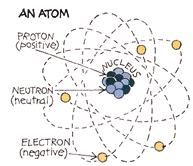
\includegraphics[width=1in]{atom.jpg},\centerline{\footnotesize{The Atom}}] The \verb+multicol+ package allows using multiple columns without starting a new page.  Using floats is not possible in a columns environment, however with the \verb+picinpar+ package, I can set a picture inside a block of text---just like you one you see here.  Isn't \LaTeX{} cool?
And now we're just filling more space, and yet more space.  
\end{window}
\closearticle


\headline{Another Headline}
This is just an example to fill up some space, but as long as I have your attention, I'll give some newspaper advice.

I suppose we could also show how an equation is type set:
\begin{displaymath}
x=\frac{-b\pm\sqrt{b^2-4ac}}{2a}
\end{displaymath}
and there you have it.  

\lipsum[1-4]

\closearticle

\end{multicols}

\end{document}